% !TeX root = Bericht_main.tex
In dieser Aufgabe betrachten wir nochmals die KDR-Gleichung bei sehr geringer Diffusion. Im Gegensatz zu vorherigen Lösungsansätzen verwenden wir nun DG-Ansatzelemente.

\begin{figure}[H]
	\centering
	\captionabove{Verlauf der Masse und der Outflowrate bei Diffusion $0.000001$}
	\subfigure[Masse]{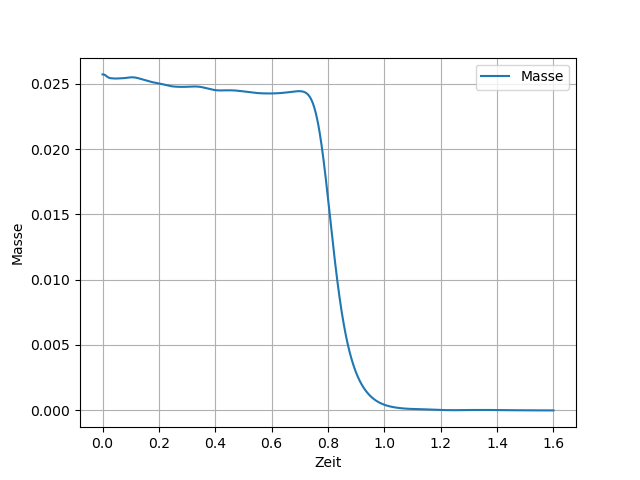
\includegraphics[width=0.49\textwidth]{../Aufgabe38/plotmass.png}}	
	\subfigure[Outflowrate]{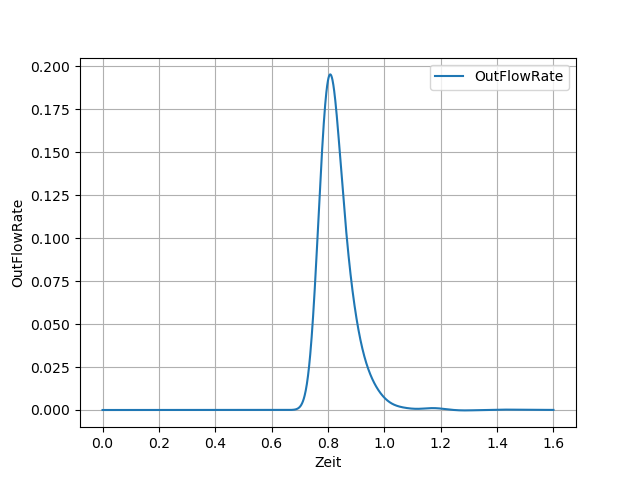
\includegraphics[width=0.49\textwidth]{../Aufgabe38/plotoutflowrate.png}}
\end{figure}

Wie man anhand des Verlaufes der Masse gut erkennen kann, eignen sich die DG-Ansatzelemente insgesamt relativ gut zum Lösen der KDR-Gleichung. Allerdings entstehen hier zu Beginn (bis $t=0.7$) leichte Oszillationen. Dies können wir anhand der zugehörigen Lösungsplots erkennen.

\begin{figure}[H]
	\centering
	\captionabove{Lösungsplots}
	\subfigure[Zeitpunkt $t=0.3$]{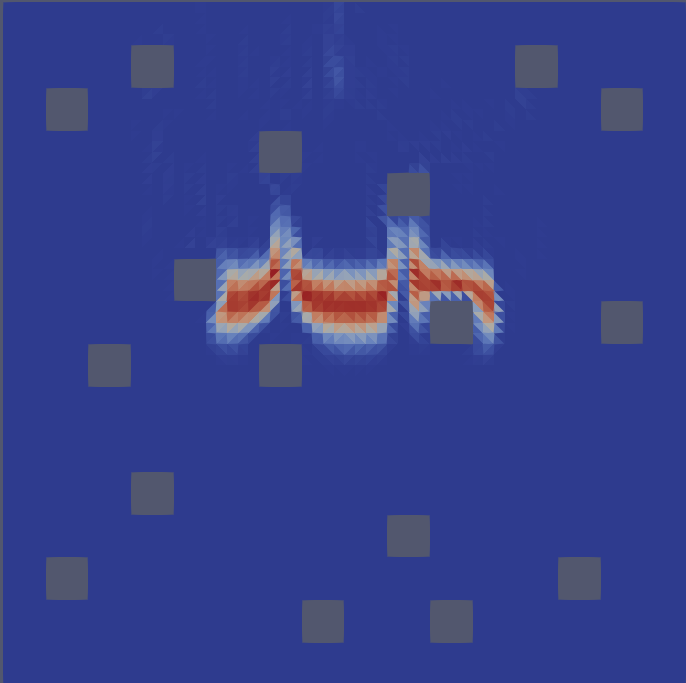
\includegraphics[width=0.49\textwidth]{../Aufgabe38/Zeit0_3.png}}	
	\subfigure[Zeitpunkt $t=0.5$]{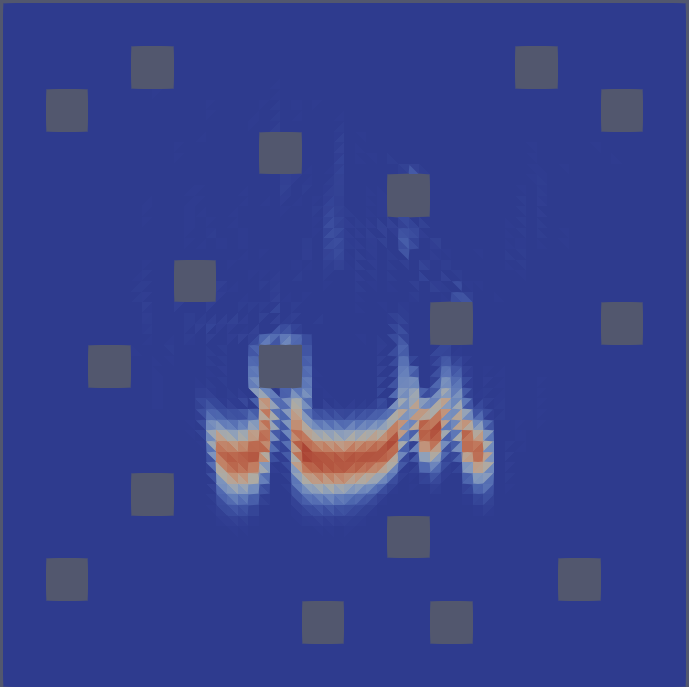
\includegraphics[width=0.49\textwidth]{../Aufgabe38/Zeit0_5.png}}
\end{figure}